\chapter{Results}

\section{Testbed Configuration}

\subsection{Minimal Testbed}

To begin testing, a testbed consisting of two similar computers was set up. These two nodes, served as both storage servers and metadata servers. This setup is relatively simple compared to large HPC clusters, which typically have dedicated storage and metadata nodes. Both nodes are identical in terms of hardware and software specifications.

\subsubsection{Hardware Specifications}
\begin{table}[H]
    \centering
    \caption{Hardware Specifications}
    \label{tab:node_specs}
    \begin{tabularx}{\textwidth}{|X|X|}
        \hline
        \textbf{Model} & MSI Z97-G55 \\
        \hline
        \textbf{CPU Model} & Intel Core i5-4590 @ 3.30GHz x 4 \\
        \hline
        \textbf{Memory} & 2 x 4GB DDR3 @ 1600MHz \\
        \hline
        \textbf{Storage} & 4 TB HDD - 250 GB SSD\\
        \hline
        \textbf{PCIe Version} & 3.0 \\
        \hline
        \textbf{PCIe Lanes} & - \\
        \hline
        \textbf{PCIe NTB} & - \\
        \hline
        \textbf{HDD Interface} & SATA 6 Gb/s \\
        \hline
        \textbf{HDD Cache} & 64MB \\
        \hline
        \textbf{HDD Throughput Max} & 180 MB/S \\
        \hline
        \textbf{HDD Average Data Rate} & 146 MB/S \\
        \hline
        \textbf{HDD Avarage Latency} & 5.16 ms \\
        \hline
    \end{tabularx}
\end{table}

\subsubsection{Software Specifications}
\begin{table}[H]
    \centering
    \caption{Software Specifications}
    \label{tab:software_specs}
    \begin{tabularx}{\textwidth}{|X|X|}
        \hline

        \textbf{Operating System} & Ubuntu 22.04.5 \\
        \hline
        \textbf{Kernel Version} & 6.8.0-52-generic \\
        \hline
        \textbf{BeeGFS Version} & 7.4.5\\ % Fill in
        \hline
        \textbf{eXpressWare Version} & x.x.x \\
        \hline
    \end{tabularx}
\end{table}

\subsubsection{Storage Configuration}
\begin{table}[H]
    \centering
    \caption{Storage Configuration}
    \label{tab:storage_specs}
    \begin{tabularx}{\textwidth}{|l|X|X|X|}
        \hline
        \textbf{Device} & \textbf{Type} & \textbf{Size} & \textbf{Purpose} \\
        \hline
        sda1 & Partition & 37.3 GB (ext4) & Unused \\
        sda2 & Partition & 149 GB (ext4) & BeeGFS metadata \\
        sda3 & Partition & 3.5 TB (XFS) & BeeGFS data \\
        nvme0n1 & NVMe SSD & 232.9 GB (ext4) & OS \\
        \hline
    \end{tabularx}
\end{table}

\subsection{Scaled Testbed}

\subsubsection{Hardware Specifications}

\begin{table}[H]
    \centering
    \caption{Hardware Specifications}
    \label{tab:node_specs}
    \begin{tabularx}{\textwidth}{|X|X|}
        \hline
        \textbf{Model} &  \\
        \hline
        \textbf{CPU Model} &  \\
        \hline
        \textbf{Memory} &  \\
        \hline
        \textbf{Storage} & \\
        \hline
        \textbf{PCIe Version} &  \\
        \hline
        \textbf{PCIe Lanes} &  \\
        \hline
        \textbf{PCIe NTB} & \\
        \hline
        \textbf{SSD Interface} & \\
        \hline
        \textbf{SSD Cache} &  \\
        \hline
        \textbf{SSD Throughput Max} &  \\
        \hline
        \textbf{SSD Average Data Rate} &  \\
        \hline
        \textbf{SSD Avarage Latency} & \\
        \hline
    \end{tabularx}
\end{table}

\subsubsection{Software Specifications}

\begin{table}[H]
    \centering
    \caption{Software Specifications}
    \label{tab:software_specs}
    \begin{tabularx}{\textwidth}{|X|X|}
        \hline

        \textbf{Operating System} &  \\
        \hline
        \textbf{Kernel Version} &  \\
        \hline
        \textbf{BeeGFS Version} & \\ % Fill in
        \hline
        \textbf{eXpressWare Version} &  \\
        \hline
    \end{tabularx}
\end{table}

\subsubsection{Storage Configuration}

\section{Minimal Testbed Results}

\subsection{Throughput vs. Block Size}

Initial performance testing was conducted using two nodes equipped with traditional hard disk drives (HDDs). FIO was used to measure sequential and random read/write performance across various block sizes. In this setup, there were two BeeGFS storage servers, each backed by an HDD with a theoretical maximum throughput of 180 MB/s and an average data rate of 146 MB/s, resulting in an expected combined average of approximately 292 MB/s.

For both sequential reads and writes, IPoPCIe and SuperSockets reached a throughput ceiling of around 260 MB/s, while Ethernet peaked just above 150 MB/s. Output from the \path{sar} tool showed that both disks were operating at 99.7\% utilization, indicating that the throughput bottleneck lies at the disk level.

Sequential read and write operations performed better than random access, which is expected for HDDs. This is because random access requires the disk to move its read/write head to different locations, which takes more time. In contrast, sequential access reads or writes data in order, allowing the disk to work more efficiently.

\begin{figure}[H]
    \centering
    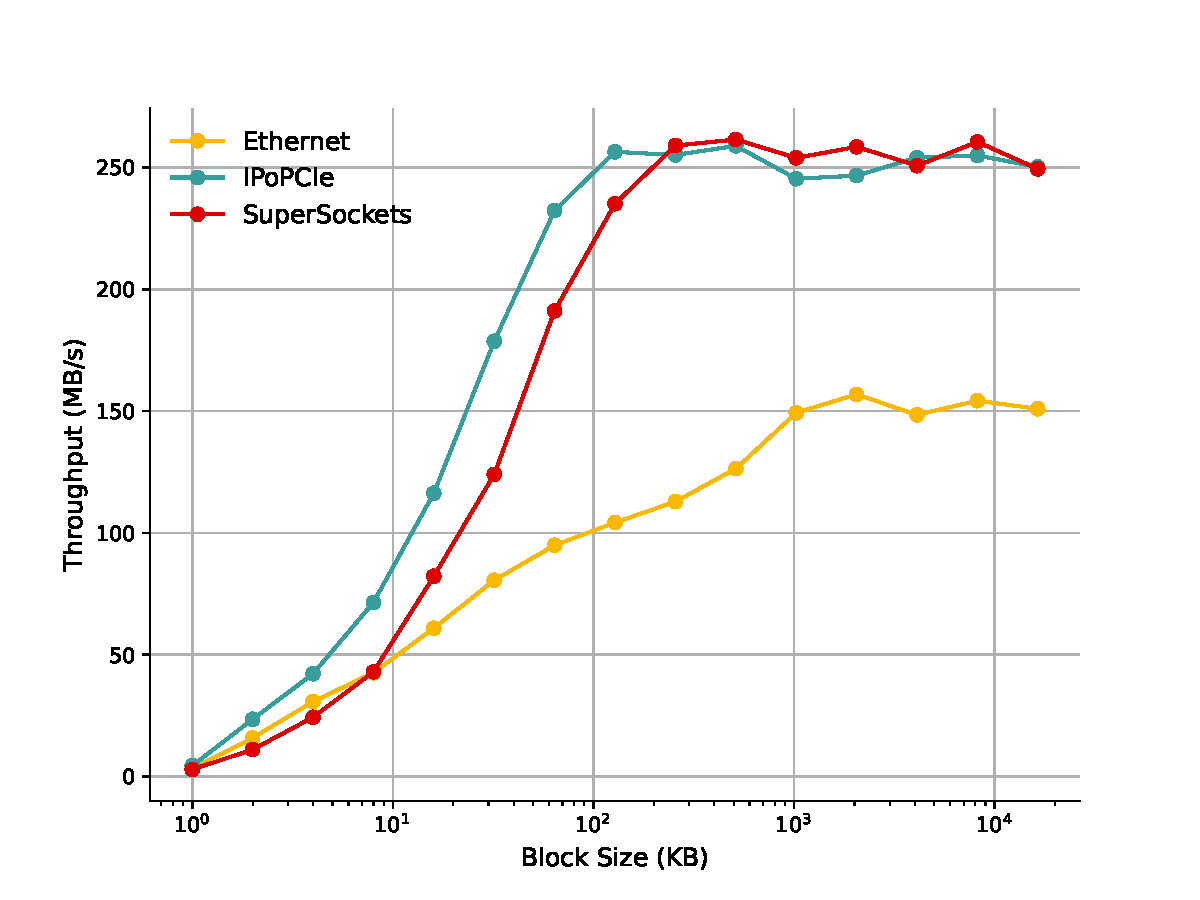
\includegraphics[width=0.99\textwidth]{fig/img/fio/throughput_vs_bs_write_seq_ssocks.pdf}
    \caption{HDD - Throughput vs. Block Size (Sequential Write)}
    \label{fig:hdd_tp_bs_seqread}
\end{figure}
\begin{figure}[H]
    \centering
    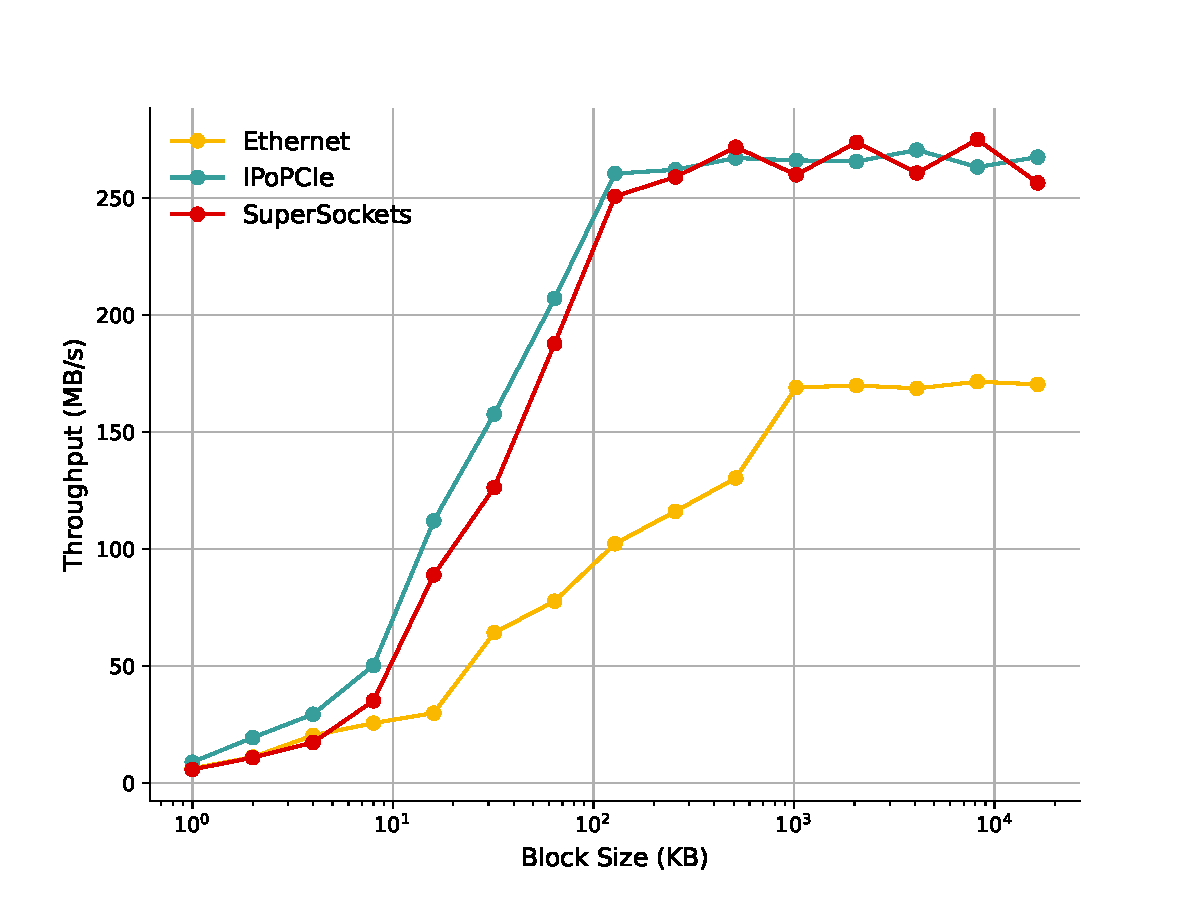
\includegraphics[width=0.99\textwidth]{fig/img/fio/throughput_vs_bs_read_seq_ssocks.pdf}
    \caption{HDD - Throughput vs. Block Size (Sequential Read)}
    \label{fig:hdd_tp_bs_seqread}
\end{figure}

\begin{figure}[H]
    \centering
    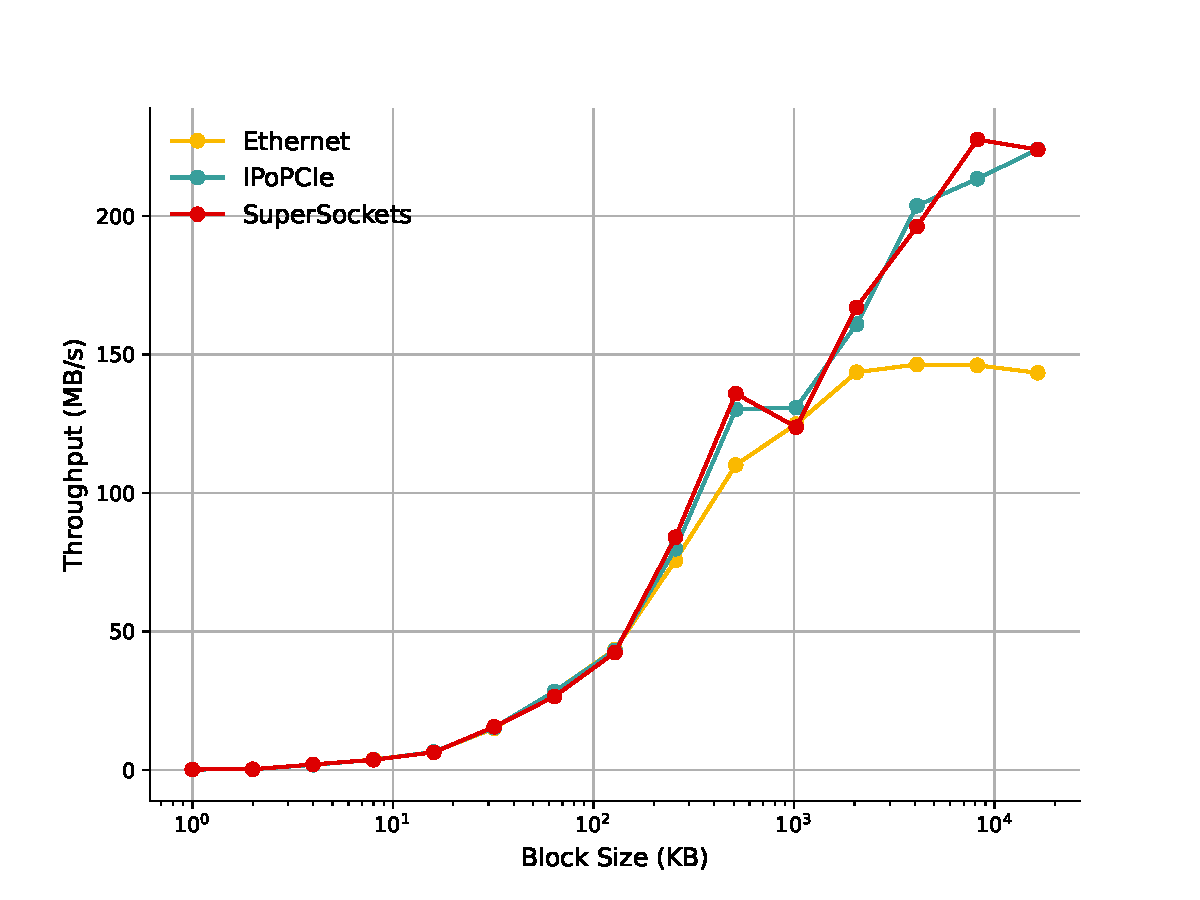
\includegraphics[width=0.99\textwidth]{fig/img/fio/throughput_vs_bs_write_rand_ssocks.pdf}
    \caption{HDD - Throughput vs. Block Size (Random Write)}
    \label{fig:hdd_tp_bs_seqread}
\end{figure}

\begin{figure}[H]
    \centering
    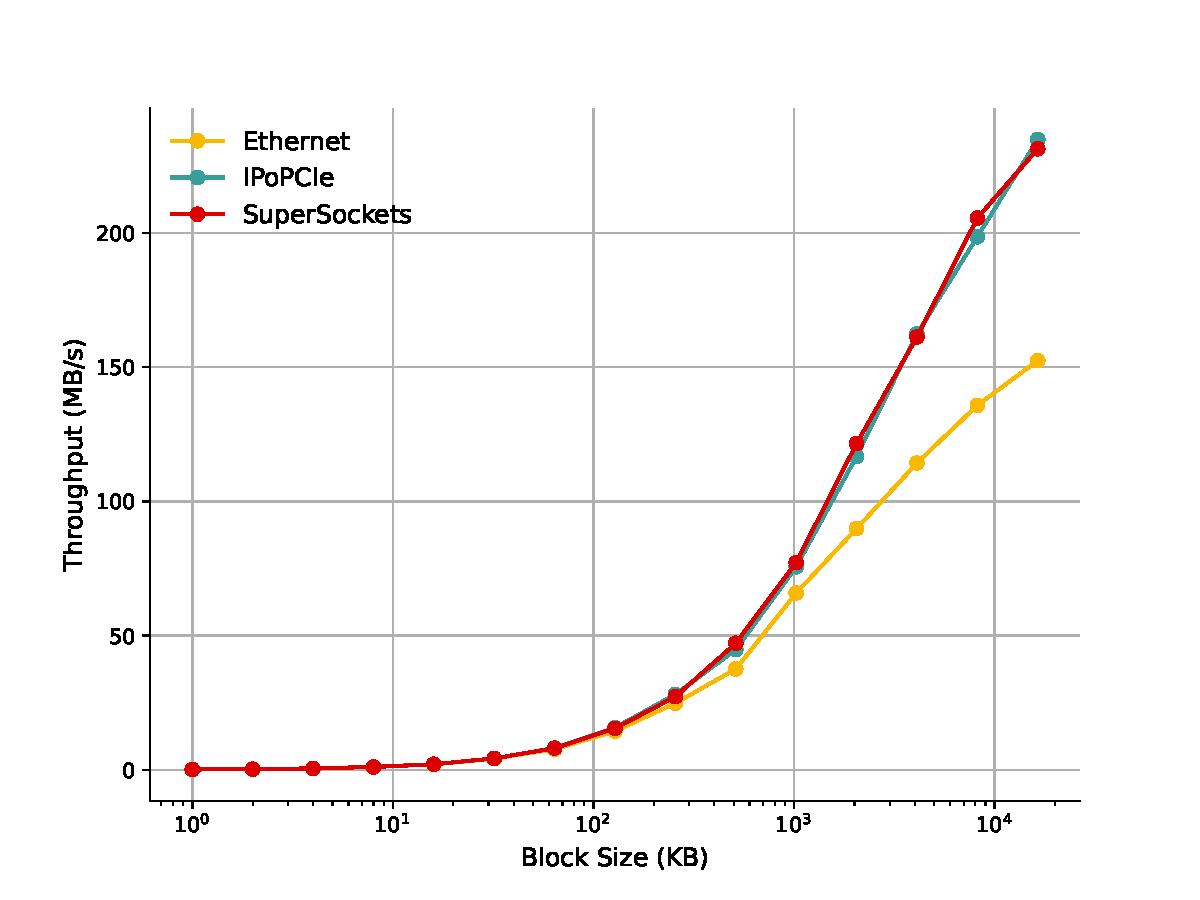
\includegraphics[width=0.99\textwidth]{fig/img/fio/throughput_vs_bs_read_rand_ssocks.pdf}
    \caption{HDD - Throughput vs. Block Size (Random Read)}
    \label{fig:hdd_tp_bs_seqread}
\end{figure}

\section{Scaled Testbed Results}

Currently empty.